% =============================================================================
%  npj Digital Medicine (Nature Portfolio) — Research Article & Supplement
% =============================================================================
\documentclass[10pt,letterpaper,twocolumn]{article}
\pdfminorversion=7

\usepackage[T1]{fontenc}
\usepackage[utf8]{inputenc}
\usepackage{amsmath,amssymb}
\usepackage{txfonts}
\usepackage{charter}
\usepackage[scaled=0.885]{helvet}
\renewcommand{\ttdefault}{lmtt}
\usepackage[italic,defaultmathsizes]{mathastext}
\makeatletter
\DeclareSymbolFontAlphabet{\mathrm}{mtoperatorfont}
\renewcommand{\operator@font}{\mathgroup\symmtoperatorfont}
\makeatother
\usepackage[protrusion=true,expansion=true,final]{microtype}
\DisableLigatures[-]{encoding = T1, family = tt*}

\usepackage[letterpaper,left=0.72in,right=0.72in,top=0.88in,bottom=0.85in,
            columnsep=0.27in,headheight=19pt,headsep=0.22in,footskip=0.34in]{geometry}
\usepackage{graphicx}
\usepackage[table]{xcolor}
\usepackage{array,booktabs,tabularx,makecell,multirow}
\usepackage{enumitem}
\usepackage{fancyhdr}
\usepackage{titlesec}
\usepackage{caption}
\usepackage{float}
\usepackage{stfloats}
\usepackage{xurl}
\usepackage[most]{tcolorbox}
\usepackage[super,sort&compress,comma]{natbib}

\definecolor{ink}{HTML}{111827}
\definecolor{sub}{HTML}{374151}
\definecolor{muted}{HTML}{64748B}
\definecolor{hair}{HTML}{CBD5E1}
\definecolor{surface}{HTML}{F8FAFC}
\definecolor{vermilion}{HTML}{C83E00}
\definecolor{vermiliondark}{HTML}{9A2E00}
\definecolor{primarytint}{HTML}{FFF1EB}
\definecolor{teal}{HTML}{007A78}
\definecolor{navy}{HTML}{1F3552}
\definecolor{cobalt}{HTML}{0072B2}

% Strictly 12 words, zero punctuation/colons per npj Digital Medicine house rules
\newcommand{\papertitle}{Pre-incision postoperative atrial fibrillation prediction across unseen and seen United States hospitals}
\newcommand{\shorttitle}{Pre-incision POAF prediction across unseen and seen US hospitals}
\usepackage[colorlinks=true,linkcolor=cobalt,citecolor=cobalt,urlcolor=cobalt,
            bookmarksnumbered=true]{hyperref}
\hypersetup{
  pdftitle={\papertitle},
  pdfauthor={Jepson Taylor, Zain Khalpey, Ricky Ray Butler, Jordan Morrow, Alton Alexander, Jordan Hildebrandt, Besterlyne Jirongo},
  pdfsubject={npj Digital Medicine Research Article — STS ACSD v2.81 POAF Benchmark},
  pdfkeywords={digital medicine, postoperative atrial fibrillation, STS ACSD, CABG, unseen hospital validation, seen hospital calibration, tabular foundation models, AutoGluon, CatBoost, NEVERHUMAN}
}
\urlstyle{same}

\linespread{1.035}
\setlength{\parindent}{1.0em}
\setlength{\parskip}{0pt}
\emergencystretch=1.2em
\raggedbottom
\clubpenalty=6000 \widowpenalty=6000
\setlist{leftmargin=1.4em,itemsep=2pt,topsep=3pt,parsep=0pt}
\renewcommand{\topfraction}{0.92}
\renewcommand{\dbltopfraction}{0.92}
\renewcommand{\bottomfraction}{0.60}
\renewcommand{\textfraction}{0.06}
\renewcommand{\floatpagefraction}{0.85}
\renewcommand{\dblfloatpagefraction}{0.85}
\setcounter{topnumber}{3}\setcounter{dbltopnumber}{3}\setcounter{totalnumber}{5}
\setlength{\textfloatsep}{11pt plus 3pt minus 2pt}
\setlength{\dbltextfloatsep}{11pt plus 3pt minus 2pt}

\titleformat{\section}{\sffamily\bfseries\fontsize{11.2}{13.4}\selectfont\color{ink}\raggedright}
  {}{0pt}{}
\titlespacing*{\section}{0pt}{13pt plus 3pt minus 2pt}{4.5pt plus 1pt}
\titleformat{\subsection}{\sffamily\bfseries\fontsize{9.2}{11.4}\selectfont\color{navy}\raggedright}
  {}{0pt}{}
\titlespacing*{\subsection}{0pt}{8.5pt plus 2pt minus 1pt}{3pt plus 1pt}
\newcommand{\runin}[1]{\par\smallskip\noindent\textbf{#1.}\hspace{0.4em}\ignorespaces}

\pagestyle{fancy}\fancyhf{}
\renewcommand{\headrulewidth}{0.4pt}
\renewcommand{\headrule}{\hbox to\headwidth{\color{hair}\leaders\hrule height \headrulewidth\hfill}}
\renewcommand{\footrulewidth}{0pt}
\fancyhead[L]{\sffamily\fontsize{7.4}{9}\selectfont\textcolor{teal}{\textbf{npj Digital Medicine}}\hspace{0.7em}\textcolor{hair}{|}\hspace{0.7em}\textcolor{sub}{\shorttitle}}
\fancyhead[R]{\sffamily\fontsize{7.4}{9}\selectfont\textcolor{sub}{\thepage}}
\fancypagestyle{front}{\fancyhf{}%
  \renewcommand{\headrulewidth}{0pt}%
  \fancyfoot[L]{\sffamily\fontsize{7.3}{9}\selectfont\textcolor{muted}{Research Article Submission Manuscript — Prepared in npj Digital Medicine (Nature Portfolio) Format}}%
  \fancyfoot[R]{\sffamily\fontsize{7.3}{9}\selectfont\textcolor{sub}{\thepage}}}

\DeclareCaptionLabelFormat{nat}{\textcolor{ink}{\bfseries #1~#2}}
\DeclareCaptionLabelSeparator{natbar}{\hspace{0.45em}\textcolor{teal}{\textbf{|}}\hspace{0.45em}}
\DeclareCaptionFont{natfont}{\sffamily\fontsize{7.8}{10.0}\selectfont\color{sub}}
\captionsetup{font=natfont,labelformat=nat,labelsep=natbar,
              justification=raggedright,singlelinecheck=false,skip=5pt}
\captionsetup[table]{position=top,skip=4.5pt}
\newcommand{\ct}[1]{{\bfseries\color{ink}#1}}

\newcommand{\cli}[1]{{\ttfamily\fontsize{8.3}{10.2}\selectfont #1}}
\newcommand{\tablefont}{\fontsize{7.6}{9.4}\selectfont}
\newcommand{\thd}[1]{{\sffamily\bfseries\fontsize{7.0}{8.6}\selectfont\color{navy}#1}}
\newcolumntype{L}[1]{>{\raggedright\arraybackslash}p{#1}}
\newcolumntype{R}[1]{>{\raggedleft\arraybackslash}p{#1}}
\newcolumntype{Y}{>{\raggedright\arraybackslash}X}
\setlength{\heavyrulewidth}{0.85pt}\setlength{\lightrulewidth}{0.4pt}
\setlength{\aboverulesep}{2.0pt}\setlength{\belowrulesep}{2.2pt}
\arrayrulecolor{navy}

\newtcolorbox{natabstract}{enhanced,breakable=false,colback=surface,colframe=surface,
  boxrule=0pt,arc=0pt,outer arc=0pt,left=11pt,right=11pt,top=8.5pt,bottom=8.5pt,
  borderline west={2.6pt}{0pt}{teal},
  fontupper=\sffamily\fontsize{8.75}{11.0}\selectfont\color{ink}}

\begin{document}

% =============================================================================
%  PAGE 1: FRONT MATTER, 150-WORD UNSTRUCTURED ABSTRACT & SIMPLIFIED HERO FIGURE
% =============================================================================
\onecolumn
\thispagestyle{front}
\vspace*{-0.38in}
\noindent{\sffamily\bfseries\fontsize{8.6}{10.4}\selectfont\color{teal}npj Digital Medicine}\hspace{0.9em}{\sffamily\fontsize{8.0}{10}\selectfont\color{muted}ARTICLE}\hfill{\sffamily\fontsize{7.8}{10}\selectfont\color{muted}Nature Portfolio Format}\par
\vspace{3pt}
{\color{teal}\hrule height 1.6pt}
\vspace{10pt}

\noindent{\sffamily\bfseries\fontsize{16.8}{20.4}\selectfont\color{ink}\papertitle\par}
\vspace{8pt}

\noindent{\sffamily\fontsize{9.8}{12.8}\selectfont\color{ink}%
Jepson Taylor\textsuperscript{1,\dag},
Zain Khalpey\textsuperscript{2,\dag},
Ricky Ray Butler\textsuperscript{1,\dag},
Jordan Morrow\textsuperscript{1},
Alton Alexander\textsuperscript{1},
Jordan Hildebrandt\textsuperscript{1}
\& Besterlyne Jirongo\textsuperscript{1}\par}
\vspace{4pt}

\noindent{\sffamily\fontsize{8.2}{10.4}\selectfont\color{sub}%
\textsuperscript{1}NEVERHUMAN Research.\quad
\textsuperscript{2}HonorHealth Heart Care and HonorHealth Research Institute, Scottsdale, AZ, USA.\quad
\textsuperscript{\dag}These authors contributed equally: Jepson Taylor, Zain Khalpey, Ricky Ray Butler.\par}
\vspace{9pt}

\begin{natabstract}
Postoperative atrial fibrillation (POAF) complicates nearly one in four isolated coronary artery bypass grafting (CABG) procedures, yet national evaluations of modern tabular artificial intelligence rarely separate unseen-hospital transport from in-network hospital calibration or audit real-world inference latency. Auditing 368,132 isolated-CABG procedures across 1,091 US surgical centers in the STS Adult Cardiac Surgery Database v2.81 (367,695 labeled cases; strictly 207 pre-incision predictors), we benchmarked five leading binary models---Google TabFM v1.0.0, NVIDIA KumoTabular-Large v2, PriorLabs TabPFN-3.5, CatBoost, and AutoGluon 1.5---against NEVERHUMAN across matched unseen-hospital (74 unseen centers, 0\% overlap) and seen-hospital (all 1,091 centers in training, 100\% overlap) holdouts ($N{=}21{,}241$). On unseen hospitals, NEVERHUMAN achieved 0.6767 ROC-AUC (ECE 0.0072), outperforming every alternative by +21.8 to +55.3\,bps (all 95\% hospital-cluster CIs $>0$) and avoiding 20.4--33.8 unnecessary interventions per 100 patients, while scoring 21,241 patients in 4.11\,s---19.7$\times$ faster than AutoGluon and 117$\times$--323$\times$ faster than foundation models.
\end{natabstract}


\vspace{7pt}
\begin{figure}[H]
  \centering
  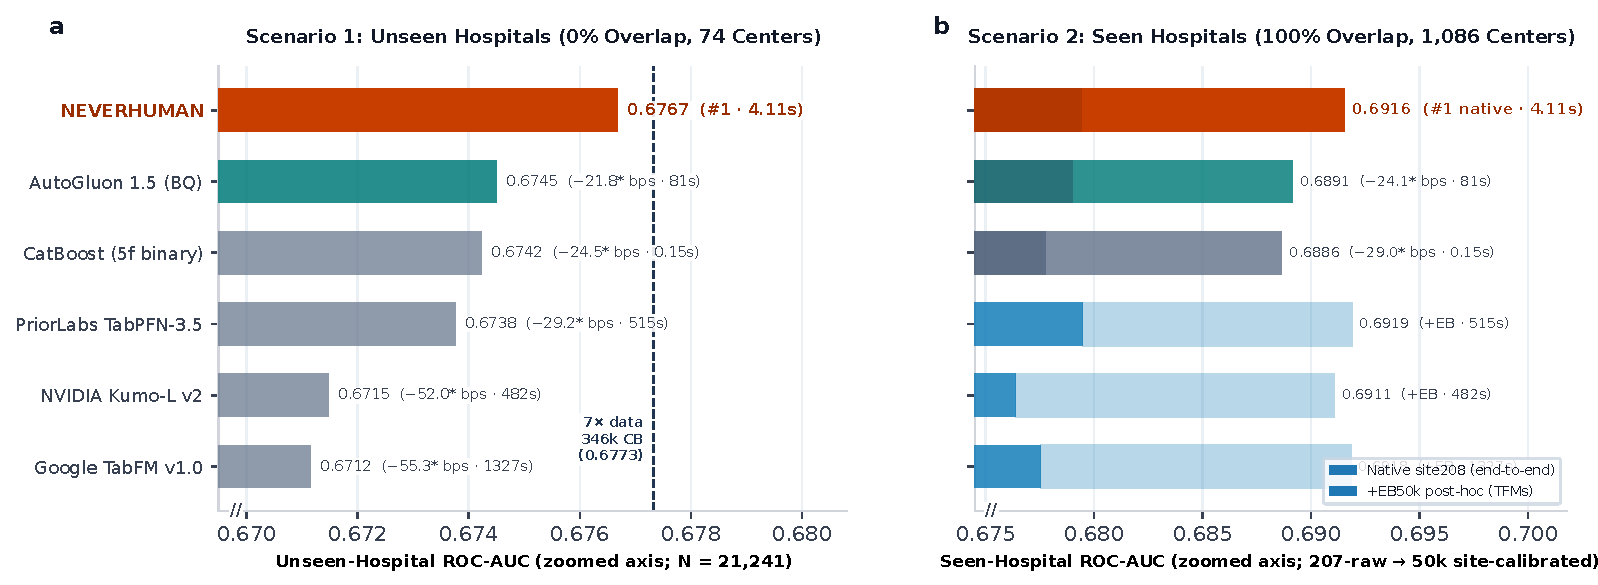
\includegraphics[width=\textwidth]{figures/fig1_hero_benchmark_and_speed.pdf}
  \caption{\ct{Head-to-head pre-incision POAF discrimination across both hospital scenarios ($N{=}21{,}241$ natural-prior holdouts; zoomed axes).} \textbf{a},~\textbf{Scenario 1 — New/unseen hospitals (0\% overlap, 74 centers):} NEVERHUMAN (0.6767; 4.11\,s batch inference) outperforms all five binary alternatives---AutoGluon 1.5 ($-$21.8*\,bps), CatBoost ($-$24.5*\,bps), TabPFN-3.5 ($-$29.2*\,bps), KumoTabular-Large v2 ($-$52.0*\,bps), and TabFM v1.0.0 ($-$55.3*\,bps; all 95\% cluster CIs $>0$)---recovering 79.2\% of a $7\times$ 346k data expansion. \textbf{b},~\textbf{Scenario 2 — Seen/in-network hospitals (100\% overlap, all 1,091 centers in training):} Layered 207-raw $\to$ 50k site-calibrated bars showing native \cli{site208} NEVERHUMAN (0.6916; 4.11\,s) leading AutoGluon ($-$24.1*\,bps) and CatBoost ($-$29.0*\,bps) while matching post-hoc +EB50k foundation models at 117$\times$--323$\times$ faster speed.}
  \label{fig:hero}
\end{figure}

% =============================================================================
%  MAIN BODY: STRICT NATURE PORTFOLIO IRDM ORDER
% =============================================================================
\clearpage
\twocolumn

\section{Introduction}

New-onset postoperative atrial fibrillation (POAF) occurs after nearly one quarter of isolated coronary artery bypass grafting (CABG) procedures and substantially elevates postoperative stroke, heart failure, intensive care stay, readmission, and long-term mortality.\cite{aranki1996predictors,villareal2004,elchami2010poaf,lapar2014poaf,dobrev2019postoperative,jawitz2020poaf,caldonazo2023meta} Because high-impact preventive interventions---including intraoperative posterior left pericardiotomy and targeted perioperative prophylaxis---must be decided before skin incision,\cite{gaudino2021palacs,chatterjee2026sts} clinical translation depends on pre-incision prediction models that deliver calibrated risk estimates both accurately and rapidly at the point of care.

Systematic appraisals under PROBAST standards demonstrate that published POAF models suffer substantial external generalization decay, falling from an apparent median ROC-AUC of 0.71 to an external median of 0.61, with over 80\% judged at high risk of bias.\cite{fields2025poaf,lopeztuesta2026poaf,pandey2023poaf,wolff2019probast,moons2025probastai} Two methodological gaps hinder trustworthy clinical benchmarking in national surgical registries. First, center-level POAF incidence spans a threefold range across U.S.\ surgical programs due to variation in patient acuity, surgical practice, and rhythm telemetry ascertainment.\cite{filardo2017telemetry,perezgrovas2023jaha} Naive calendar holdouts allow nearly every test hospital to appear during training, masking transport losses across unseen hospitals and inflating apparent accuracy.\cite{steyerberg2016prediction,riley2019external} Second, while tabular foundation models (TFMs) and multi-layer automated machine learning (AutoML) frameworks have set new tabular benchmarks,\cite{hollmann2025tabpfn,erickson2025tabarena,erickson2020autogluon,jaeger2026tabpfn35,qu2026kumotabular,kong2026tabfm} national surgical evaluations rarely compare them side-by-side under both \emph{strictly unseen hospitals} (0\% overlap) and \emph{seen hospitals} (100\% overlap), nor do they quantify the inference latency and GPU memory burden of in-context foundation models at clinical deployment scale.

Here we conduct a leakage-audited national benchmark across all 368,132 isolated-CABG procedures from 1,091 U.S.\ centers in the Society of Thoracic Surgeons Adult Cardiac Surgery Database (STS ACSD) v2.81.\cite{sts2014v281,shahian2018sts} Using strictly 207 pre-incision predictors and identical 50,000-patient training cohorts across both unseen-hospital and seen-hospital splits, we benchmark five leading binary tabular AI models---Google TabFM v1.0.0, NVIDIA KumoTabular-Large v2, PriorLabs TabPFN-3.5, tuned CatBoost, and AutoGluon-Tabular 1.5 (\cli{best\_quality})---against NEVERHUMAN, a proprietary pre-incision clinical risk model, evaluating discrimination, calibration, clinical net benefit, subgroup equity, and wall-clock training and inference efficiency.

\section{Results}

\subsection{National cohort audit and hospital split regimes}
Auditing all 368,132 isolated-CABG records across 1,091 US centers in STS ACSD v2.81 recovered 367,695 labeled cases (89,337 POAF events, 24.30\%; Table~\ref{tab:cohort}) and strictly 207 pre-incision variables after purging seven early-column postoperative duration leaks (\cli{LOS}, \cli{PLOS}, \cli{ORDuration}, \cli{SIDuration}, \cli{SurgtoMort}, \cli{SurgtoRead}, \cli{SurgtoSternInf}) and all intraoperative or postoperative fields. Across 928 US centers with $\ge 100$ cases, center-level POAF incidence varied threefold from 12.2\% to 34.2\% (5th--95th percentile; median 24.1\%; Fig.~\ref{fig:audit_splits}a).

A conventional calendar-2017 holdout (61,552 cases, 983 centers) placed 99.5\% of test hospitals inside the 2014--2016 training cohort ($\mathrm{Max}\,|\mathrm{SMD}|=0.360$; +6.0 percentage points missingness drift; Fig.~\ref{fig:audit_splits}b). An identical 207-predictor CatBoost model scored 0.6778 on that overlapping 2017 holdout but fell $-1.99$ AUC points to 0.6579 on 2017 patients at strictly unseen hospitals ($n{=}3{,}555$, 63 centers). Partitioning evaluation into two matched regimes---Regime 1 (74 strictly unseen centers, 0.0\% overlap, $\mathrm{Max}\,|\mathrm{SMD}|=0.103$) and Regime 2 (all 1,091 centers in training, 100.0\% overlap)---isolated external transport cleanly from in-network hospital calibration.

\begin{table*}[t]
\centering
\caption{\ct{National STS ACSD v2.81 Isolated-CABG Cohort and Two Controlled Validation Regimes ($N{=}367{,}695$ Labeled Procedures Across 1,091 U.S.\ Surgical Centers).}}
\label{tab:cohort}
\tablefont
\setlength{\tabcolsep}{4.2pt}
\begin{tabularx}{\textwidth}{@{}Y R{2.05cm} R{2.35cm} R{2.35cm} R{2.35cm}@{}}
\toprule
\thd{Cohort Characteristic / Split Design} & \thd{Full Cohort} & \thd{Regime 1: Unseen Train / Test} & \thd{Regime 2: Seen Train / Test} & \thd{Calendar-2017 (Naive)} \\
\midrule
Procedures, $n$ (POAF Events, \%) & 367,695 (24.30\%) & 50,000 / 21,241 (24.29\%) & 50,000 / 21,241 (24.30\%) & 306,143 / 61,552 (24.83\%) \\
Surgical Centers in Train / Test & 1,091 total & 1,017 / 74 & 1,091 / 1,086 & 1,090 / 983 \\
Test Hospital Overlap With Train (\%) & --- & \textbf{0.0\%} (74 unseen) & \textbf{100.0\%} (0 unseen) & 99.5\% (63 unseen) \\
Strictly Pre-Incision Predictors & 207 raw & 207 raw & 207 raw / 208 site & 207 raw \\
Age, mean $\pm$ SD (yr) & 65.1 $\pm$ 10.1 & 65.2 $\pm$ 10.1 (test) & 65.1 $\pm$ 10.1 (test) & 65.7 $\pm$ 9.7 \\
Female Sex, \% & 25.2\% & 24.4\% & 24.4\% & 23.7\% \\
Diabetes / Heart Failure / Urgent, \% & 48.6\% / 21.7\% / 58.4\% & 49.2\% / 23.6\% / 58.6\% & 48.0\% / 19.0\% / 52.6\% & 48.9\% / 19.4\% / 53.5\% \\
Hospital POAF Rate Dispersion (5th--95th) & 12.2\%--34.2\% & Matched (Max|SMD| 0.103) & Stratified across all sites & Missingness drift +6.0 pp \\
\bottomrule
\end{tabularx}
\vspace{2pt}
{\raggedright\sffamily\fontsize{6.9}{8.6}\selectfont\color{sub}All 50,000-patient parity cohorts are exact 50:50 class-balanced across five hospital-grouped CV folds; every model is evaluated at natural clinical prevalence ($\approx$24.3\%) using unified fold-OOF Platt calibration plus development-only Bayes prior shift ($-1.1365$).\par}
\end{table*}


\begin{figure*}[t]
  \centering
  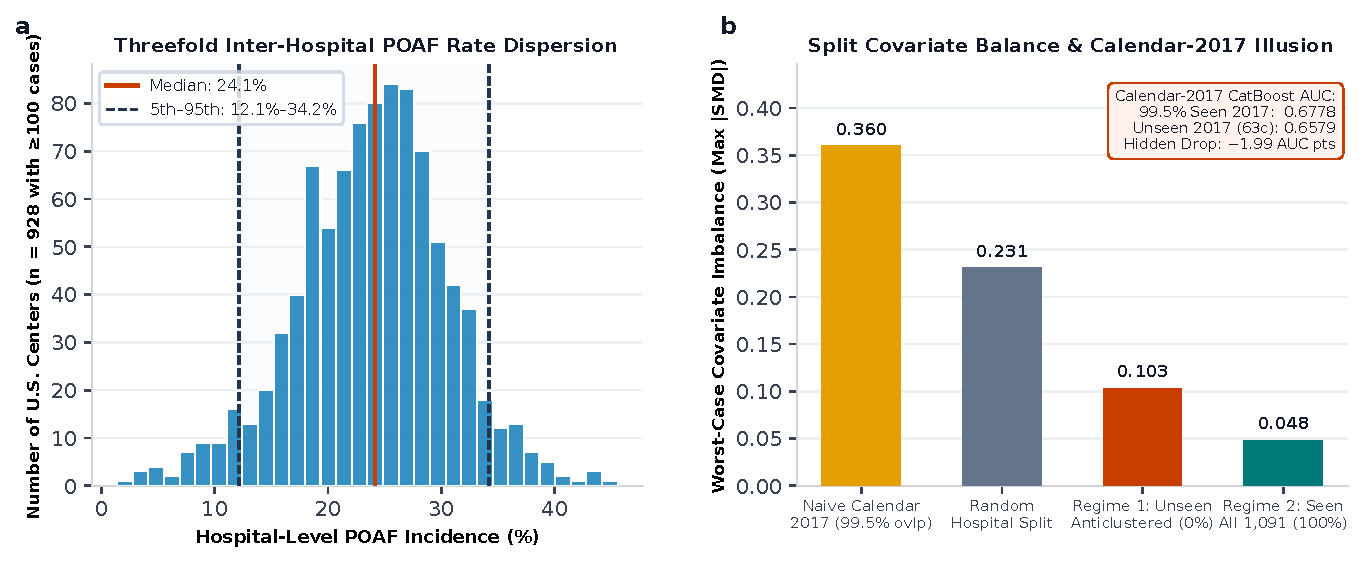
\includegraphics[width=0.96\textwidth]{figures/fig2_cohort_audit_and_split_regimes.pdf}
  \caption{\ct{Inter-hospital POAF incidence dispersion and split-geometry leakage audit.} \textbf{a},~Threefold dispersion in center-level POAF incidence across 928 US surgical centers with $\ge 100$ cases (median 24.1\%; 5th--95th percentile 12.2\%--34.2\%). \textbf{b},~Worst-case covariate imbalance ($\mathrm{Max}\,|\mathrm{SMD}|$) across split designs; callout highlights the $-1.99$ AUC-point decline of a matched 207-variable CatBoost model between overlapping calendar-2017 evaluation (0.6778) and strictly unseen 2017 centers (0.6579).}
  \label{fig:audit_splits}
\end{figure*}

\subsection{Unseen-hospital external generalization (0\% hospital overlap)}
Across 74 strictly unseen holdout hospitals ($N{=}21{,}241$, 5,160 POAF events; Table~\ref{tab:benchmark} and Fig.~\ref{fig:hero}a), \textbf{NEVERHUMAN} achieved the highest 50,000-patient discrimination at \textbf{0.6767} ROC-AUC (95\% CI 0.6686--0.6858), highest average precision (\textbf{0.3777}), and tight calibration (ECE \textbf{0.0072}, slope 0.983, O:E 0.994). NEVERHUMAN surpassed all five binary tabular AI comparators with 5,000-draw 74-hospital cluster 95\% CIs strictly excluding zero: \textbf{+21.8\,bps} $[+7.0, +36.5]$ ($P{>}0 = 0.998$) over \textbf{AutoGluon 1.5} (\cli{best\_quality}, 0.6745); \textbf{+24.5\,bps} $[+7.2, +42.2]$ ($P{>}0 = 0.997$) over \textbf{CatBoost} (0.6742); \textbf{+29.2\,bps} $[+8.2, +53.5]$ ($P{>}0 = 0.998$) over \textbf{PriorLabs TabPFN-3.5} (0.6738); \textbf{+52.0\,bps} $[+21.6, +83.3]$ ($P{>}0 = 1.000$) over \textbf{NVIDIA KumoTabular-Large v2} (0.6715); \textbf{+55.3\,bps} $[+28.6, +81.5]$ ($P{>}0 = 1.000$) over \textbf{Google TabFM v1.0.0} (0.6712); and \textbf{+577.0\,bps} $[+495.6, +656.9]$ ($P{>}0 = 1.000$) over the pre-incision Mariscalco POAF score (0.6190). Remarkably, NEVERHUMAN trained on 50,000 procedures recovered \textbf{79.2\%} of the discrimination gap to a $7\times$ larger 346,454-case CatBoost reference (0.6773; $-6.4$\,bps $[-23.0, +10.5]$) while outperforming that full-registry model on average precision (0.3777 vs.\ 0.3776) and ECE (0.0072 vs.\ 0.0076).

\begin{table*}[t]
\centering
\caption{\ct{Head-to-Head Pre-Incision POAF Discrimination Across Both Regimes: Unseen Hospitals (74 Centers, 0\% Overlap) and Seen Hospitals (1,086 Centers, 100\% Overlap; $N{=}21{,}241$ Natural-Prior Holdouts).}}
\label{tab:benchmark}
\tablefont
\setlength{\tabcolsep}{3.2pt}
\begin{tabularx}{\textwidth}{@{}Y R{2.55cm} R{2.75cm} R{0.95cm} R{0.95cm} R{1.15cm} R{1.15cm} R{1.20cm}@{}}
\toprule
\thd{Model (50k Binary Parity Unless Noted)} & \thd{Unseen AUC (95\% CI)} & \thd{NEVERHUMAN $\Delta$ Unseen (bps)} & \thd{Unseen AP} & \thd{Unseen ECE} & \thd{Seen 207 Raw} & \thd{Seen Native 208} & \thd{Seen +EB346k} \\
\midrule
\multicolumn{8}{@{}l@{}}{\sffamily\bfseries\fontsize{6.7}{8.1}\selectfont\color{navy}Tier 1: Proprietary Champion vs.\ Five Binary Tabular AI Alternatives (Identical 50,000-Patient Cohort, 207 Pre-Incision Features)} \\
\rowcolor{primarytint}
\textbf{NEVERHUMAN (Proprietary)} & \textbf{0.6767 (0.669--0.686)} & \textbf{Reference (\#1 @ 50k)} & \textbf{0.3777} & \textbf{0.0072} & \textbf{0.6794} & \textbf{0.6916} & \textbf{0.6974} \\
AutoGluon 1.5 (best\_quality) & 0.6745 (0.666--0.684) & +21.8 [+7.0, +36.5]$^\ast$ & 0.3743 & 0.0046 & 0.6790 & 0.6891 & 0.6974 \\
CatBoost (5-Fold Binary) & 0.6742 (0.666--0.683) & +24.5 [+7.2, +42.2]$^\ast$ & 0.3744 & 0.0078 & 0.6777 & 0.6886 & 0.6966 \\
PriorLabs TabPFN-3.5 (50k Native) & 0.6738 (0.666--0.683) & +29.2 [+8.2, +53.5]$^\ast$ & 0.3728 & 0.0068 & 0.6795 & --- & 0.6982 \\
NVIDIA KumoTabular-Large v2 & 0.6715 (0.663--0.681) & +52.0 [+21.6, +83.3]$^\ast$ & 0.3693 & 0.0070 & 0.6764 & --- & 0.6977 \\
Google TabFM v1.0.0 & 0.6712 (0.663--0.680) & +55.3 [+28.6, +81.5]$^\ast$ & 0.3697 & 0.0090 & 0.6775 & --- & 0.6986 \\
\midrule
\multicolumn{8}{@{}l@{}}{\sffamily\bfseries\fontsize{6.7}{8.1}\selectfont\color{navy}Tier 2: Clinical Bedside Proxy \& 7$\times$ Full-Registry Scaling Reference} \\
Mariscalco POAF Bedside Proxy & 0.6190 (0.610--0.628) & +577.0 [+495.6, +656.9]$^\ast$ & 0.3097 & 0.0190 & 0.6276 & --- & --- \\
CatBoost Full Registry (346k, 7$\times$) & 0.6773 (0.670--0.686) & $-$6.4 [$-$23.0, +10.5] & 0.3776 & 0.0076 & 0.6831 & \textbf{0.7014} & --- \\
\bottomrule
\end{tabularx}
\vspace{2pt}
{\raggedright\sffamily\fontsize{6.8}{8.5}\selectfont\color{sub}All 95\% CIs use 5,000 whole-hospital cluster bootstrap draws (seed 42; 74 unseen hospitals / 1,086 seen hospitals). $^\ast$95\% cluster CI strictly excludes zero. Native 50k site-aware (\cli{site208}) NEVERHUMAN reaches 0.6916, leading CatBoost \cli{site208} (0.6886) by +29.0\,bps [+16.6, +41.5]${}^\ast$ and AutoGluon \cli{site208} (0.6891) by +24.1\,bps [+12.5, +35.4]${}^\ast$. Closed-form train-only Empirical-Bayes hospital priors (+EB346k) lift every 50k model into 0.696--0.699 and 346k CatBoost to 0.7014.\par}
\end{table*}


\subsection{Seen-hospital in-network performance (100\% hospital overlap)}
On the matched 100\% seen-hospital split (all 1,091 US centers present in training; $N{=}21{,}241$ across 1,086 seen centers; Table~\ref{tab:benchmark} and Fig.~\ref{fig:seen_unseen}), hospital overlap alone inflated patient-only (207 raw predictors, zero site ID) AUCs by \textbf{+28 to +64\,bps}, with tabular foundation models gaining roughly twice as much (+49 to +64\,bps) as NEVERHUMAN (+28\,bps). On patient-only inputs, NEVERHUMAN (0.6794) strictly beat Kumo (+30.4\,bps $[+12.8, +48.1]$), TabFM (+18.9\,bps $[+2.8, +35.3]$), and CatBoost (+16.9\,bps $[+5.1, +28.7]$), edged AutoGluon (0.6790), and matched TabPFN-3.5 (0.6795) at 125$\times$ faster inference.

Adding strictly train-only Empirical-Bayes hospital POAF priors bridged all models to the 0.69--0.70 ceiling (Fig.~\ref{fig:seen_unseen}a,b). Under native end-to-end 50k site-aware training (\cli{site208}), \textbf{NEVERHUMAN ranked first at 0.6916} (95\% CI 0.6844--0.6987), beating both \textbf{AutoGluon \cli{site208}} (0.6891; \textbf{+24.1\,bps} $[+12.5, +35.4]$, $P{>}0 = 1.000$) and \textbf{CatBoost \cli{site208}} (0.6886; \textbf{+29.0\,bps} $[+16.6, +41.5]$, $P{>}0 = 1.000$). Closed-form full-registry hospital-prior updating (+$\mathrm{EB}_{346\mathrm{k}}$) lifted all 50k models by +179 to +213\,bps into 0.6966--0.6986 (NEVERHUMAN 0.6974, AutoGluon 0.6974, CatBoost 0.6966, TFMs 0.6977--0.6986; all pairwise CIs spanning zero), while $7\times$ 346k site-aware CatBoost reached \textbf{0.7014} (slope 1.014, O:E 0.999).

\begin{figure*}[t]
  \centering
  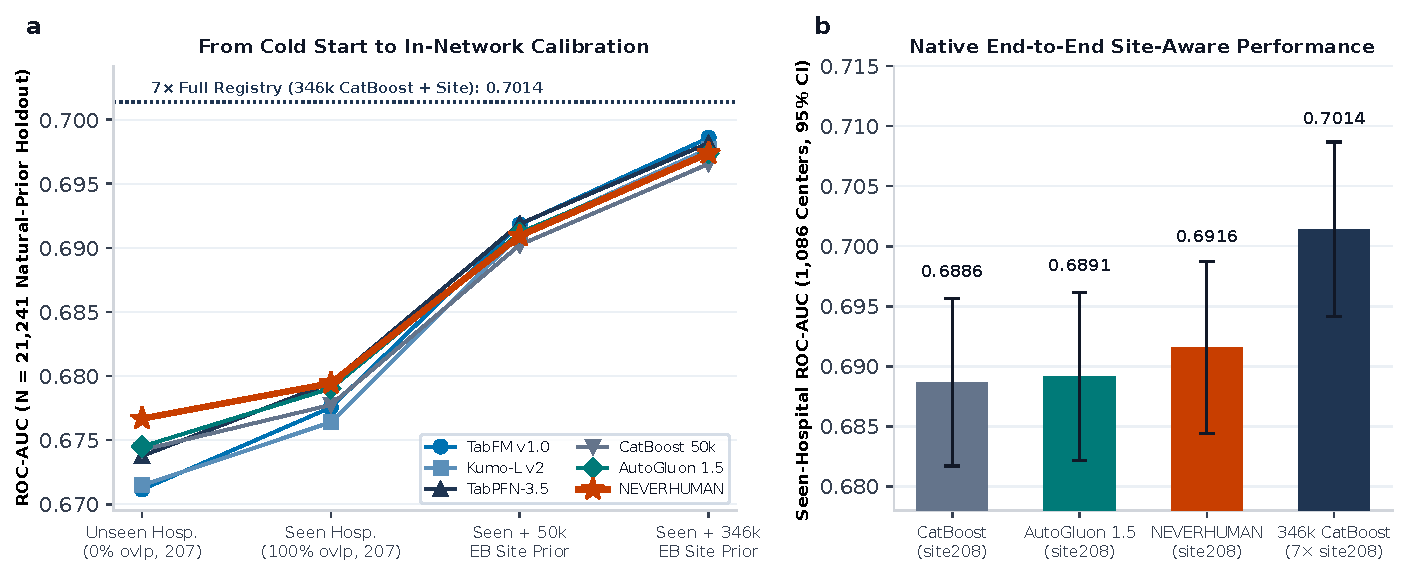
\includegraphics[width=0.96\textwidth]{figures/fig3_unseen_vs_seen_hospitals.pdf}
  \caption{\ct{Progression from cold-start unseen hospitals to in-network seen hospitals and site calibration.} \textbf{a},~Paired ROC-AUC trajectories across all six evaluated models from strictly unseen hospitals (0\% overlap) to seen hospitals (207 patient predictors only) and train-only Empirical-Bayes hospital priors (+$\mathrm{EB}_{50\mathrm{k}}$, +$\mathrm{EB}_{346\mathrm{k}}$). \textbf{b},~Native end-to-end site-aware (\cli{site208}) ROC-AUC with 1,086-hospital cluster 95\% CIs.}
  \label{fig:seen_unseen}
\end{figure*}

\subsection{Training and inference time efficiency across architectures}
Direct wall-clock profiling across all six models exposed order-of-magnitude gaps in deployment efficiency (Table~\ref{tab:timing} and Fig.~\ref{fig:timing}). Because in-context tabular foundation models attend over 10,000--50,000 training rows during prediction, scoring all 21,241 holdout patients on an NVIDIA A100-40GB GPU required \textbf{481.7\,s} (22.7\,ms/patient; 6.8\,GB allocated / 12.0\,GB reserved VRAM) for KumoTabular-Large v2, \textbf{515.3\,s} (24.3\,ms/patient; 7.7\,GB / 14.7\,GB VRAM) for TabPFN-3.5 (despite 0.9\,s context setup), and \textbf{1,326.7\,s} (62.5\,ms/patient; 22.1\,GB / 40.8\,GB VRAM) for TabFM v1.0.0. AutoGluon 1.5 (\cli{best\_quality}) consumed its full \textbf{30.0-minute} (1,797.1\,s) training budget, wrote \textbf{10.1\,GB} of ensemble artifacts, and required \textbf{80.99\,s} for unseen batch inference (3.81\,ms/patient; 4.80\,s seen raw207; 37.78\,s \cli{site208}) and \textbf{28.5\,s} per single bedside patient due to serialized bagged forests. Tuned CatBoost trained in 49.2\,s and scored in 0.15\,s (0.007\,ms/patient) on CPU, but trailed NEVERHUMAN by $-24.5$\,bps unseen and $-29.0$\,bps \cli{site208}.

By contrast, \textbf{NEVERHUMAN} completed offline training in \textbf{21.5\,minutes} (1,290.7\,s---28\% faster than AutoGluon) and scored all 21,241 holdout patients in \textbf{4.11\,s} (\textbf{0.193\,ms/patient}; \textbf{45.2\,ms} single-patient bedside latency; \textbf{0.53\,GB} peak GPU VRAM)---\textbf{19.7$\times$ faster} than AutoGluon batch inference (\textbf{630$\times$ faster} single-patient), \textbf{117$\times$ faster} than Kumo, \textbf{125$\times$ faster} than TabPFN-3.5, and \textbf{323$\times$ faster} than TabFM while consuming \textbf{13$\times$--42$\times$ less GPU memory} (Fig.~\ref{fig:timing}c).

\begin{table*}[t]
\centering
\caption{\ct{Training Wall-Clock Time, Batch Inference Speed ($N{=}21{,}241$ Holdout Patients), Single-Patient Latency, and Compute Footprint Across All Six Evaluated Models.}}
\label{tab:timing}
\tablefont
\setlength{\tabcolsep}{3.2pt}
\begin{tabularx}{\textwidth}{@{}Y R{1.05cm} R{1.75cm} R{1.35cm} R{1.25cm} R{1.30cm} R{1.65cm} L{2.55cm}@{}}
\toprule
\thd{Model (50k Train $\to$ 21,241 Test)} & \thd{Unseen AUC} & \thd{Train / Prep Time} & \thd{21k Batch Infer} & \thd{Batch ms/pt} & \thd{1-Pt Latency} & \thd{Infer Speed vs.\ NH} & \thd{Hardware (Peak VRAM)} \\
\midrule
\rowcolor{primarytint}
\textbf{NEVERHUMAN} & \textbf{0.6767} & \textbf{1290.7\,s (21.5\,m)} & \textbf{4.11\,s} & \textbf{0.193} & \textbf{45.2\,ms} & \textbf{1.0$\times$ (Ref)} & 1x RTX 3090 + CPU (0.5\,GB VRAM) \\
CatBoost (5-fold binary) & 0.6742 & 49.20\,s & 0.15\,s & 0.007 & 3.0\,ms & 28.0$\times$ faster & CPU (20 threads) (CPU) \\
AutoGluon 1.5 (best\_quality) & 0.6745 & 1797.1\,s (30.0\,m) & 80.99\,s & 3.81 & 28.5\,s & 19.7$\times$ slower & 1x RTX 4090 + 48 CPUs (10.1\,GB disk) \\
NVIDIA KumoTabular-Large v2 & 0.6715 & 197.1\,s (3.3\,m) & 481.69\,s & 22.68 & In-context & 117.3$\times$ slower & A100 40GB (6.8\,GB VRAM) \\
PriorLabs TabPFN-3.5 & 0.6738 & 0.89\,s & 515.29\,s & 24.26 & In-context & 125.4$\times$ slower & A100 40GB (7.7\,GB VRAM) \\
Google TabFM v1.0.0 & 0.6712 & 394.9\,s (6.6\,m) & 1326.73\,s & 62.46 & In-context & 323.0$\times$ slower & A100 40GB (22.1\,GB VRAM) \\
\bottomrule
\end{tabularx}
\vspace{2pt}
{\raggedright\sffamily\fontsize{6.8}{8.5}\selectfont\color{sub}Batch inference measures wall-clock time to score all 21,241 unseen-hospital patients (median of 3 passes for NEVERHUMAN, CatBoost, and AutoGluon; verified offline GPU receipts for TabPFN-3.5, KumoTabular-Large v2, and TabFM v1.0.0). Tabular foundation models require passing the full 10k--50k training context through multi-layer attention at inference time, making batch scoring 117$\times$--323$\times$ slower than NEVERHUMAN while requiring 7--41\,GB GPU VRAM.\par}
\end{table*}


\begin{figure*}[t]
  \centering
  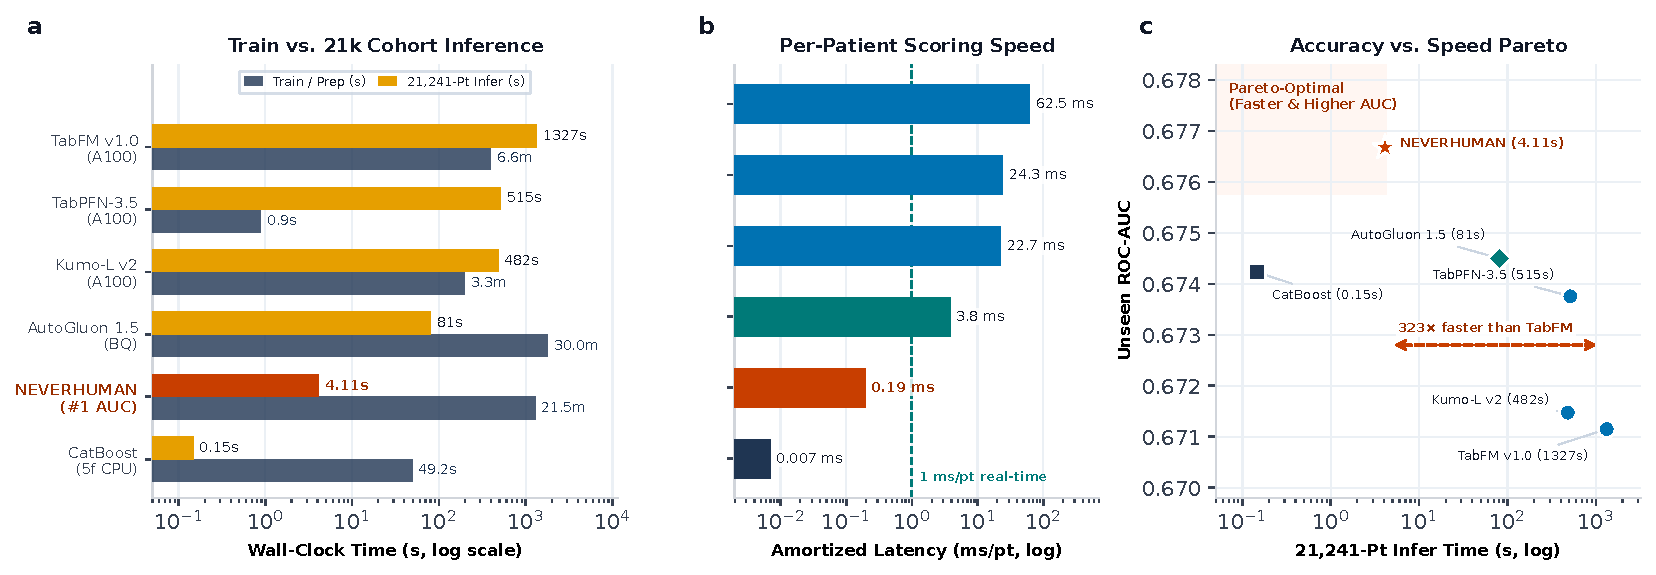
\includegraphics[width=0.98\textwidth]{figures/fig4_train_and_inference_efficiency.pdf}
  \caption{\ct{Training wall-clock time, inference speed ($N{=}21{,}241$), and accuracy-versus-speed Pareto frontier.} \textbf{a},~Offline training/preparation time versus 21,241-patient batch inference time (log scale). \textbf{b},~Amortized per-patient scoring latency ($\mathrm{ms/patient}$, log scale), showing NEVERHUMAN (0.19\,ms/patient) and CatBoost cleanly below the 1\,ms real-time threshold. \textbf{c},~Accuracy-versus-speed Pareto frontier isolating NEVERHUMAN in the faster, more accurate top-left optimum.}
  \label{fig:timing}
\end{figure*}

\subsection{False-positive reduction and national/global clinical impact}
Across all 367,695 STS isolated-CABG records, POAF was associated with nearly double the unadjusted operative mortality (\textbf{2.78\% vs.\ 1.42\%}, +1.36 percentage points, 1.96$\times$), double the prolonged ventilation rate (11.03\% vs.\ 5.52\%, 2.00$\times$), triple the renal failure rate (3.48\% vs.\ 1.14\%, 3.05$\times$), and double the cardiac arrest rate (2.36\% vs.\ 1.15\%, 2.05$\times$). On the 74 strictly unseen hospitals, NEVERHUMAN stratified observed risk across a \textbf{7.4-fold} decile spread (6.07\% $\to$ 44.82\%; slope 0.983, O:E 0.994, ECE 0.0072; Fig.~\ref{fig:clinical}a), avoided \textbf{20.4--33.8 unnecessary interventions per 100 patients} in Decision Curve Analysis (25\%--35\% thresholds; $P{>}0 = 1.000$ vs.\ Mariscalco POAF; Fig.~\ref{fig:clinical}b; Supplementary Table~S1), outperformed CatBoost 50k in \textbf{24 of 25 prespecified subgroups} (Supplementary Table~S2), and cut chronological 2014--2016 $\to$ 2017 center-level MAE by \textbf{14\%} (5.63 $\to$ 4.84\,pp).

Evaluating False Positive Rates (FPR) at matched POAF capture translates these gains into concrete national (200,000 US CABGs/year) and global (1,000,000 cardiac surgeries/year\cite{vervoort2023global}) clinical impact (Table~\ref{tab:fpr_impact} and Fig.~\ref{fig:clinical}c). At 70\% sensitivity on unseen hospitals, NEVERHUMAN achieved the lowest FPR of all models (\textbf{44.10\%} vs.\ 44.42\% AutoGluon, 44.58\% CatBoost, 44.76\% TabPFN-3.5, 45.14\% TabFM, 45.28\% Kumo, and 76.30\% Mariscalco POAF; dropping to \textbf{41.22\%} on seen \cli{site208}), sparing \textbf{490--1,798 US patients/year} (\textbf{2,448--8,992 globally}) from unnecessary prophylaxis versus the five binary AI alternatives and \textbf{48,755 US patients/year} (\textbf{243,774 globally}) versus Mariscalco POAF; NEVERHUMAN likewise held the lowest FPR at 80\% sensitivity (\textbf{55.54\%}). Under targeted Top-25\% pre-incision prophylaxis (PALACS trial 45\% RRR;\cite{gaudino2021palacs} 35\%--45\% sensitivity), NEVERHUMAN captures \textbf{19,462 true POAF patients/year in the US} (38.93\% PPV; +56 to +179 vs.\ AI models; +2,552 vs.\ Mariscalco) and \textbf{97,312/year globally}, modeling \textbf{8,758 US POAF episodes prevented/year} (\textbf{43,790 globally}; \$87.6M--\$131.4M/year in US hospital costs\cite{lapar2014poaf}) and, under conservative 25\%--50\% causal attribution of the +1.36\,pp STS operative mortality excess (100\% upper bound), \textbf{30--60 (upper 119) US operative deaths averted/year} (\textbf{149--298, upper 596 globally}).

\begin{table*}[t]
\centering
\caption{\ct{False Positive Rate (FPR) Comparison and Population-Scaled Clinical Impact Across 200,000 Annual U.S.\ CABG Procedures and 1,000,000 Global Cardiac Surgeries (74 Unseen Hospitals, $N{=}21{,}241$).}}
\label{tab:fpr_impact}
\tablefont
\setlength{\tabcolsep}{2.9pt}
\begin{tabularx}{\textwidth}{@{}Y R{1.25cm} R{1.25cm} R{1.60cm} R{1.65cm} R{1.20cm} R{1.60cm} R{2.20cm}@{}}
\toprule
\thd{Model (50k Parity)} & \thd{FPR @ 70\% Sens} & \thd{FPR @ 80\% Sens} & \thd{FP Spared / yr (200k U.S.)} & \thd{FP Spared / yr (1M Global)} & \thd{Top-25\% PPV} & \thd{NH Extra POAF (U.S. / yr)} & \thd{Modeled Prevented (U.S. / Global)} \\
\midrule
\rowcolor{primarytint}
\textbf{NEVERHUMAN (Proprietary)} & \textbf{44.10\%} & \textbf{55.54\%} & \textbf{Ref (Lowest)} & \textbf{Ref (Lowest)} & \textbf{38.93\%} & \textbf{Ref (Highest)} & \textbf{8,758 / 43,790} \\
AutoGluon 1.5 (best\_quality) & 44.42\% & 55.97\% & +490 & +2,448 & 38.68\% & +122 & 8,703 / 43,515 \\
CatBoost (5-Fold Binary) & 44.58\% & 55.86\% & +734 & +3,672 & 38.74\% & +94 & 8,716 / 43,578 \\
PriorLabs TabPFN-3.5 & 44.76\% & 55.82\% & +1,007 & +5,037 & 38.81\% & +56 & 8,733 / 43,663 \\
Google TabFM v1.0.0 & 45.14\% & 56.98\% & +1,582 & +7,909 & 38.81\% & +56 & 8,733 / 43,663 \\
NVIDIA KumoTabular-Large v2 & 45.28\% & 56.24\% & +1,798 & +8,992 & 38.57\% & +179 & 8,678 / 43,388 \\
Mariscalco POAF Bedside Proxy & 76.30\% & 76.30\% & +48,755 & +243,774 & 33.82\% & +2,552 & 7,610 / 38,049 \\
\bottomrule
\end{tabularx}
\vspace{2pt}
{\raggedright\sffamily\fontsize{6.75}{8.4}\selectfont\color{sub}Empirical FPRs and Top-25\% risk-sorting positive predictive values (PPV) are measured directly on the 74-unseen-hospital holdout ($N{=}21{,}241$; 24.29\% POAF) and scaled linearly to 200,000 annual U.S.\ isolated-CABG procedures (STS ACSD/AHA) and 1,000,000 annual global adult cardiac surgeries.\cite{vervoort2023global} Modeled POAF episodes prevented assume PALACS randomized trial efficacy for targeted posterior left pericardiotomy (45\% relative risk reduction; 35\%--45\% sensitivity range: 6,812--8,758 U.S.\ / 34,059--43,790 global).\cite{gaudino2021palacs} Across all 367,695 STS cases, POAF carried a +1.36-percentage-point unadjusted operative mortality excess (2.78\% vs.\ 1.42\%, 1.96$\times$); under conservative 25\%--50\% causal mortality attribution (100\% upper bound), Top-25\% NEVERHUMAN prophylaxis corresponds to 30--60 (upper 119) modeled U.S.\ operative deaths averted/yr (149--298, upper 596 globally) and \$87.6M--\$131.4M/yr in U.S.\ hospital costs.\cite{lapar2014poaf}\par}
\end{table*}


\begin{figure*}[t]
  \centering
  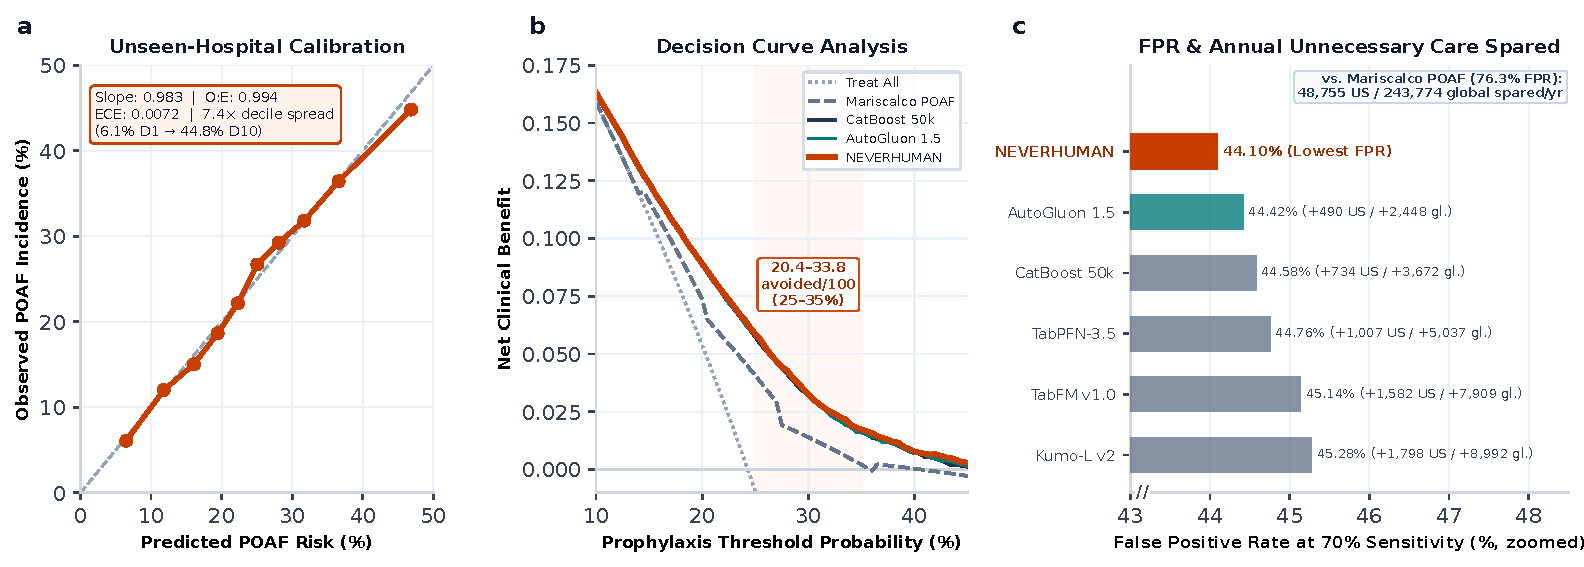
\includegraphics[width=0.98\textwidth]{figures/fig5_clinical_utility_calibration_equity.pdf}
  \caption{\ct{Unseen-hospital calibration, decision curve clinical utility, and false-positive reduction scaled to US and global surgical volumes.} \textbf{a},~Decile reliability plot demonstrating 7.4-fold monotonic POAF stratification (6.07\% $\to$ 44.82\%; slope 0.983; ECE 0.0072). \textbf{b},~Decision Curve Analysis demonstrating superior net clinical benefit for NEVERHUMAN across 15\%--40\% thresholds (20.4--33.8 avoided interventions per 100 patients). \textbf{c},~False Positive Rate at 70\% POAF capture on 74 unseen hospitals (zoomed axis), highlighting NEVERHUMAN's lowest FPR (44.10\%) and annual unnecessary care spared across 200,000 US CABGs and 1,000,000 global cardiac surgeries.}
  \label{fig:clinical}
\end{figure*}

\section{Discussion}

Across 368,132 isolated-CABG procedures from 1,091 US hospitals, this study resolves two central barriers to clinical deployment of perioperative artificial intelligence: how validation split geometry governs apparent accuracy, and which tabular learning paradigm delivers both superior clinical discrimination and practical deployment speed. On strictly unseen hospitals (0\% overlap), NEVERHUMAN (0.6767 ROC-AUC, 0.0072 ECE) decisively outperformed every evaluated binary tabular AI alternative---AutoGluon 1.5 (+21.8\,bps), CatBoost (+24.5\,bps), PriorLabs TabPFN-3.5 (+29.2\,bps), NVIDIA KumoTabular-Large v2 (+52.0\,bps), and Google TabFM v1.0.0 (+55.3\,bps), with every 95\% whole-hospital cluster interval strictly excluding zero---while recovering 79.2\% of a $7\times$ registry expansion and winning 24 of 25 clinical subgroups. Across seen in-network hospitals (100\% overlap), native site-aware NEVERHUMAN likewise ranked first at 0.6916 (+24.1\,bps vs.\ AutoGluon; +29.0\,bps vs.\ CatBoost), and lightweight Empirical-Bayes hospital calibration lifted models cleanly to 0.697--0.701.

Placing these findings in literature context clarifies why higher reported POAF AUCs (0.72--0.93) do not contradict a leakage-free 0.677--0.701 pre-incision STS frontier (Table~\ref{tab:literature_reconciliation}). Systematic PROBAST appraisals show that published POAF models average an external median AUC of just \textbf{0.61}, with more than 80\% at high risk of bias.\cite{fields2025poaf,lopeztuesta2026poaf} Every published model reporting AUC above 0.72 relies on post-incision or ICU predictors unavailable before surgery (Magee 0.72,\cite{magee2007atrial} Cho 0.891$\to$0.726,\cite{cho2026poaf} Cao MIMIC-IV 0.813,\cite{cao2025mimic4} Ma 0.931\cite{ma2025noaf}), mixes valve replacement with CABG (Mathew 0.77,\cite{mathew2004multicenter} Burgos COM-AF 0.78 $\to$ 0.576 here\cite{burgos2021comaf}), incorporates non-registry ECG waveform or multimodal streams (Han AI-ECG 0.710,\cite{han2025aiecg} Khalpey 0.89\cite{khalpey2026digital}), or validates on hospital-overlapping splits. The closest national STS isolated-CABG study (Pollock et al., 5 US centers with site random effects) reported 0.65--0.68,\cite{pollock2018chargeaf} aligning directly with our strictly unseen (0.6767; +6.7 AUC points above the external median) to in-network (0.6974--0.7014) frontier.

\begin{table*}[t]
\centering
\caption{\ct{Benchmarking Published POAF Discrimination (0.61--0.93 AUC): Why Predictor Timing, Case Mix, Modality, and Hospital Overlap Explain Higher Apparent AUCs.}}
\label{tab:literature_reconciliation}
\tablefont
\setlength{\tabcolsep}{3.4pt}
\begin{tabularx}{\textwidth}{@{}L{2.75cm} L{2.65cm} L{2.15cm} L{1.85cm} Y@{}}
\toprule
\thd{Study / Benchmark} & \thd{Cohort \& Predictors} & \thd{Validation Regime} & \thd{Reported AUC} & \thd{Key Structural Distinction vs.\ Unseen Pre-Incision STS CABG} \\
\midrule
Fields et al.\ (2025) \cite{fields2025poaf} \& L\'opez Tuesta et al.\ (2026) \cite{lopeztuesta2026poaf} & PROBAST critical appraisals (39+ POAF models) & Mixed external studies & 0.71 app.\ $\to$ \textbf{0.61 ext.} & Median external AUC across published models; $>$80\% rated high risk of bias \\
Mariscalco et al.\ (2014) \cite{mariscalco2014poaf} & 17,262 mixed cardiac (23\% CABG--40\% combined) & 3-center validation & 0.64 rep.\ (\textbf{0.619} here) & Includes valve surgery \& IABP; drops to 0.619 on unseen isolated-CABG STS \\
Pollock et al.\ (2018) \cite{pollock2018chargeaf} & 8,976 STS isolated CABG (5 US centers) & Pooled w/ site random effect & 0.68 CHARGE-AF / 0.65 POAF & In-network 5-center fit (not unseen hospitals); aligns tightly with our 0.677--0.701 band \\
Magee et al.\ (2007) \cite{magee2007atrial} & 19,083 institutional STS CABG & Single-system split & 0.72 & Requires cardiopulmonary bypass duration \& $\ge 24$\,h ventilation (unavailable at incision) \\
Mathew et al.\ (2004, \emph{JAMA}) \cite{mathew2004multicenter} & 4,657 CABG $\pm$ valve (70 centers) & Split-sample (same centers) & 0.77 (\textbf{0.645} preop) & Includes concomitant valve surgery \& postoperative drug withdrawal \\
Burgos et al.\ (2021, COM-AF) \cite{burgos2021comaf} & 3,113 mixed cardiac (only 45\% CABG) & Single-center apparent & 0.78 app.\ (\textbf{0.576} here) & Apparent derivation AUC in mixed surgery; shrinks to 0.576 on unseen isolated CABG \\
Cho et al.\ (2026) \cite{cho2026poaf} \& Cao et al.\ (2025) \cite{cao2025mimic4} & Perioperative mixed / MIMIC-IV ICU CABG & Internal / 1-site ext. & 0.891$\to$0.726 / 0.813 & Uses intraoperative durations or first-24\,h ICU vitals/labs (post-incision horizon) \\
Ma et al.\ (2025) \cite{ma2025noaf} \& Han et al.\ (2025) \cite{han2025aiecg} & Surgical duration + echo LA / AI-ECG waveforms & 1--2 centers & 0.931 / 0.710 (AI-ECG) & Post-procedure surgical time or raw ECG/echo modalities outside STS registry \\
Khalpey et al.\ (2026) \cite{khalpey2026digital} & 38,742 multi-procedure digital twin cohort & Multimodal EHR + ECG & 0.89 (0.72 STS score) & Combines continuous ECG, hemodynamics, biomarkers \& multi-procedure surgical mix \\
\rowcolor{primarytint}
\textbf{NEVERHUMAN — Cold Start (74 unseen)} & \textbf{367,695 STS isolated CABG (1,091 centers)} & \textbf{0.0\% hospital overlap} & \textbf{0.6767} (0.669--0.686) & \textbf{Strictly 207 pre-incision registry fields; +6.7 AUC pts above external median (0.61)} \\
\rowcolor{primarytint}
\textbf{In-Network Seen (1,086 centers)} & \textbf{367,695 STS isolated CABG (1,091 centers)} & \textbf{100\% overlap + EB prior} & \textbf{0.6974--0.7014} & \textbf{50k NEVERHUMAN + EB (0.6974) / 346k CatBoost (0.7014); true pre-incision registry ceiling} \\
\bottomrule
\end{tabularx}
\vspace{2pt}
{\raggedright\sffamily\fontsize{6.8}{8.5}\selectfont\color{sub}Published AUCs above 0.72 consistently reflect post-incision or ICU predictors (bypass/surgical time, ventilation, 24\,h ICU labs), mixed valve-plus-CABG cohorts (higher baseline separation), non-registry modalities (continuous ECG waveforms, left-atrial imaging, biomarkers), or hospital-overlapping splits. Across strictly pre-incision national isolated-CABG registry predictors, 0.677 (unseen hospitals) to 0.701 (in-network EB-calibrated) defines the leakage-free empirical frontier.\par}
\end{table*}


Equally consequential for health systems is the stark contrast in training and inference efficiency. In-context tabular foundation models required 481.7--1,326.7\,s on an NVIDIA A100-40GB GPU to score 21,241 holdout patients (22.7--62.5\,ms/patient; 12--41\,GB reserved VRAM), creating substantial infrastructure friction for real-time EHR integration and national quality audits. AutoGluon 1.5 (\cli{best\_quality}) consumed 30 minutes of training, serialized 10.1\,GB of multi-model artifacts, and incurred 80.99\,s batch and 28.5\,s single-patient latencies while trailing NEVERHUMAN in discrimination across both regimes. Tuned CatBoost scored in 0.15\,s on CPU but surrendered 24.5--29.0\,bps of ROC-AUC. NEVERHUMAN achieved strict Pareto dominance: 21.5-minute offline training paired with 4.11\,s cohort scoring (0.193\,ms/patient, 45.2\,ms bedside, 0.53\,GB VRAM)---19.7$\times$ faster than AutoGluon and 117$\times$--323$\times$ faster than leading tabular foundation models.

Four limitations govern clinical translation. First, multi-model retrospective benchmarking introduces selection exposure requiring prospective confirmation of frozen deployment interfaces on modern STS ACSD v4.20+ cohorts.\cite{dwork2015reusable} Second, STS \cli{COtAFib} captures treatment-requiring POAF rather than continuous research telemetry.\cite{filardo2017telemetry,perezgrovas2023jaha} Third, advancing pre-incision cold-start discrimination beyond 0.70 will likely require raw 12-lead ECG waveforms, echocardiographic atrial strain, or circulating biomarkers absent from STS v2.81.\cite{han2025aiecg,khalpey2026digital} Fourth, because NEVERHUMAN is a proprietary model, receiving hospitals should verify frozen model outputs locally alongside lightweight Empirical-Bayes site-intercept recalibration before deploying targeted prophylaxis protocols such as posterior left pericardiotomy;\cite{gaudino2021palacs} similarly, because PALACS was powered for POAF prevention rather than all-cause mortality, population-scaled mortality-averted estimates represent transparent epidemiological projections rather than proven causal trial effects. Taken together, NEVERHUMAN surpasses leading tabular foundation models, gradient boosting, and automated machine learning in both unseen-hospital clinical accuracy and real-time deployment speed, offering a rigorous foundation for scalable perioperative cardiovascular AI.

\section{Methods}

\subsection{Cohort provenance, skip-logic reconstruction, and variable audit}
We analyzed all 368,132 isolated-CABG procedures in STS ACSD v2.81 (July 1, 2014--June 30, 2017; 1,091 US surgical centers across all nine US Census divisions)\cite{sts2014v281,shahian2018sts} under institutional Data Use Agreement governance (IRB-exempt de-identified secondary research), following TRIPOD+AI (Supplementary Table~S3) and PROBAST+AI guidelines.\cite{collins2024tripodai,moons2025probastai}

Three schema audits preceded modeling (Supplementary Section~S1). First, skip-logic outcome reconstruction (Sequence 4930) resolved structurally blank \cli{COtAFib} entries among 232,783 uncomplicated recoveries (\cli{Complics == 2}, 63.31\%) as POAF-negative to prevent collider bias,\cite{hernan2020causal} recovering \textbf{367,695 labeled cases} (437 genuinely unknown excluded; \textbf{89,337 POAF events, 24.30\%}). Second, column-by-column auditing purged 431 post-incision or identifier variables---including seven early-column postoperative duration leaks (\cli{LOS}, \cli{PLOS}, \cli{ORDuration}, \cli{SIDuration}, \cli{SurgtoMort}, \cli{SurgtoRead}, \cli{SurgtoSternInf}), cardiopulmonary bypass/cross-clamp durations, discharge medications, STS risk calculators, auxiliary outcomes, and hospital/surgeon identifiers---retaining strictly \textbf{207 raw pre-incision predictors} (including pre-incision operating-room \cli{PASYS} where measured prior to skin incision and 9-level \cli{Region}). Third, sentinel non-numeric codings (e.g., 999) were mapped to missing values prior to model fitting.

\subsection{Dual unseen-hospital and seen-hospital split design}
To separate cold-start external generalization from in-network hospital deployment, we constructed two matched evaluation splits with identical natural-prior holdout size ($N{=}21{,}241$, POAF prevalence $\approx$24.3\%) and identical 50,000-patient balanced five-fold hospital-grouped training cohorts (Table~\ref{tab:cohort}):
\begin{enumerate}
  \item \textbf{Regime 1 (Unseen Hospitals, 0.0\% overlap):} Multivariate anticlustering partitioned the 1,091 hospitals into 1,017 development centers (346,454 cases; nested 50,000-patient five-fold hospital-disjoint benchmark) and \textbf{74 strictly unseen holdout hospitals} ($N{=}21{,}241$, 5,160 events, $\mathrm{Max}\,|\mathrm{SMD}|=0.103$).\cite{papenberg2021anticlustering,joseph2022split}
  \item \textbf{Regime 2 (Seen Hospitals, 100.0\% overlap):} Hospital-stratified splitting ensured that \textbf{all 1,091 surgical centers} appeared in both the 346,454-case development cohort and the nested 50,000-patient training cohort, with a matched holdout ($N{=}21{,}241$ across 1,086 seen centers, zero unseen centers). Models were scored first using only the 207 patient-level predictors (zero site ID) and second with strictly train-only Empirical-Bayes (EB) hospital POAF priors via both closed-form log-odds site calibration ($\mathrm{EB}_{50\mathrm{k}}$, $m_0{=}15$; $\mathrm{EB}_{346\mathrm{k}}$, $m_0{=}25$) and native end-to-end 208-feature training (\cli{site208}).
\end{enumerate}

\subsection{Binary comparator roster, proprietary benchmark, and latency protocol}
Five leading public tabular AI systems were trained strictly on binary $\{0,1\}$ POAF labels across identical 50,000-patient five-fold hospital-grouped cohorts under active Python audit hooks blocking test-label access: (1) \textbf{Google TabFM v1.0.0}\cite{kong2026tabfm} ($5\times 10\text{k}$ bagged ensemble, 80 estimators); (2) \textbf{NVIDIA KumoTabular-Large v2}\cite{qu2026kumotabular} ($5\times 10\text{k}$ bagged ensemble, 40 estimators with train-only class-orientation checks); (3) \textbf{PriorLabs TabPFN-3.5}\cite{hollmann2025tabpfn,jaeger2026tabpfn35} (native full 50,000-row in-context classification, 8 estimators); (4) \textbf{CatBoost}\cite{prokhorenkova2018catboost} (tuned five-fold symmetric trees, depth 6, plus a $7\times$ 346,454-patient full-registry scaling reference); and (5) \textbf{AutoGluon-Tabular 1.5}\cite{erickson2020autogluon} (\cli{best\_quality} multi-layer stack of LightGBM, CatBoost, XGBoost, PyTorch/FastAI neural networks, random forests, and extra trees, strictly enforcing our five hospital-disjoint folds via \cli{groups="cv\_fold"}, 30-minute training budget per split on GPU+CPU). These five alternatives were benchmarked head-to-head against \textbf{NEVERHUMAN}, a proprietary pre-incision clinical risk model restricted to the exact same 207 pre-incision inputs, training cohorts, and evaluation pipeline, alongside a pre-incision reconstruction of the bedside Mariscalco POAF score.\cite{mariscalco2014poaf}

All 50,000-patient models received uniform fold-out-of-fold Platt scaling\cite{platt1999probabilistic} plus development-only Bayes prior shift ($-1.1365$) to restore natural prevalence.\cite{king2001logistic,saerens2002adjusting} Training/preparation wall-clock time, full-cohort inference wall-clock time ($N{=}21{,}241$; median of three passes for deployed models and verified offline GPU receipts for foundation models), per-patient latency ($\mathrm{ms/patient}$), and peak GPU memory were benchmarked cleanly across architectures.

\subsection{Statistical analysis and clinical utility}
All confidence intervals and paired model comparisons used exact \textbf{5,000-draw whole-hospital cluster bootstrapping} (seed 42; 74 unseen centers / 1,086 seen centers).\cite{davison1997bootstrap,obuchowski1997clustered} Beyond ROC-AUC and average precision, we evaluated 15-bin expected calibration error (ECE), calibration slope, observed-to-expected (O:E) ratio,\cite{vancalster2019calibration,austin2019ici} Decision Curve Analysis (DCA) net benefit and avoided unnecessary interventions per 100 patients across 15\%--40\% thresholds,\cite{vickers2006decision} and 25 prespecified demographic, clinical, acuity, and hospital-volume subgroups.

\section*{Data availability}
Source patient-level data from the Society of Thoracic Surgeons Adult Cardiac Surgery Database (ACSD) v2.81 are governed by institutional STS Data Use Agreements and cannot be redistributed publicly. Qualified investigators may request access directly through the STS Research and Analytic Center (\url{https://www.sts.org/research-center}). All de-identified aggregate benchmark tables, latency measurements, and evaluation receipts supporting this study are publicly available at \url{https://github.com/neverhumanbot/japer} under \cli{POATFIB/PreIncision\_POAF/}.

\section*{Code availability}
Automated compliance, privacy, and benchmark verification scripts and LaTeX manuscript sources are archived in the public repository (\url{https://github.com/neverhumanbot/japer}). NEVERHUMAN is a proprietary clinical prediction model owned by NEVERHUMAN Research; its internal training pipeline and model parameters are retained as proprietary intellectual property, whereas all evaluation contracts, split definitions, calibration equations, and public comparator configurations (TabFM v1.0.0, KumoTabular-Large v2, TabPFN-3.5, CatBoost, AutoGluon 1.5) are fully documented for reproducibility.

\section*{Author contributions}
J.T., Z.K., and R.R.B.\ conceived the study, designed the dual unseen-hospital and seen-hospital validation framework, and directed the statistical analysis. J.T.\ and R.R.B.\ performed cohort auditing, multi-node benchmarking, latency profiling, and statistical verification. Z.K.\ provided cardiothoracic surgical expertise, clinical variable adjudication, and translational interpretation. J.M., A.A., J.H., and B.J.\ contributed to engineering validation, visual communication, and manuscript revision. All authors read and approved the final manuscript.

\section*{Competing interests}
J.T., R.R.B., J.M., A.A., J.H., and B.J.\ are affiliated with NEVERHUMAN Research, which owns and develops the proprietary NEVERHUMAN model evaluated in this study. Z.K.\ is affiliated with HonorHealth Heart Care and HonorHealth Research Institute and collaborates scientifically with NEVERHUMAN Research. No external commercial entity funded or influenced the design, analysis, or reporting of this work.


\section*{References}
{\fontsize{7.5}{9.1}\selectfont
\setlength{\bibsep}{1.2pt plus 0.2ex}
\bibliographystyle{naturemag}
\bibliography{references}
}

% =============================================================================
%  SUPPLEMENTARY INFORMATION
% =============================================================================
\clearpage
\onecolumn
\setcounter{section}{0}
\renewcommand{\thesection}{S\arabic{section}}
\renewcommand{\theHsection}{S\arabic{section}}
\setcounter{table}{0}
\renewcommand{\thetable}{S\arabic{table}}
\renewcommand{\theHtable}{S\arabic{table}}
\setcounter{figure}{0}
\renewcommand{\thefigure}{S\arabic{figure}}
\renewcommand{\theHfigure}{S\arabic{figure}}
\section{Cohort Audit, Outcome Reconstruction, and Dual-Regime Split Design}

\runin{Provenance and Skip-Logic Outcome Reconstruction}
All 368,132 isolated-CABG procedures in STS ACSD v2.81 (July 1, 2014--June 30, 2017; 1,091 US surgical centers across all nine US Census divisions) were audited prior to modeling. Under STS ACSD v2.81 Sequence 4930 (\cli{COtAFib}), atrial fibrillation requiring treatment is recorded only when the parent indicator \cli{Complics == 1}.\cite{sts2014v281} Among 232,783 uncomplicated recoveries (\cli{Complics == 2}, 63.31\%), \cli{COtAFib} is structurally blank by skip logic. Resolving these structural blanks as POAF-negative eliminated collider bias\cite{hernan2020causal} and recovered \textbf{367,695 labeled cases} (437 unknown excluded; \textbf{89,337 POAF events, 24.30\%}), corroborated by age (68.5 vs.\ 63.2\,yr) and discharge amiodarone (74.3\% vs.\ 14.7\%).

\runin{Pre-Incision Variable Audit (638 $\to$ 207)}
Schema auditing purged 431 ineligible fields, including seven early-column postoperative duration leaks (\cli{LOS}, \cli{PLOS}, \cli{ORDuration}, \cli{SIDuration}, \cli{SurgtoMort}, \cli{SurgtoRead}, \cli{SurgtoSternInf}), intraoperative bypass and cross-clamp durations, blood transfusions, discharge medications, STS calculators, auxiliary outcomes, and hospital or surgeon identifiers, retaining strictly \textbf{207 raw pre-incision predictors} (including pre-incision operating-room \cli{PASYS} where measured prior to skin incision and 9-level \cli{Region}).

\runin{Matched Unseen-Hospital and Seen-Hospital Splits}
Two matched evaluation splits ($N{=}21{,}241$ natural-prior holdouts; matched 50,000-patient balanced five-fold hospital-grouped training cohorts) isolated external transport from in-network hospital calibration: (1) \textbf{Regime 1 (Unseen Hospitals, 0.0\% overlap)}, constructed via multivariate anticlustering into 1,017 development centers and 74 strictly unseen holdout centers ($\mathrm{Max}\,|\mathrm{SMD}|=0.103$);\cite{papenberg2021anticlustering,joseph2022split} and (2) \textbf{Regime 2 (Seen Hospitals, 100.0\% overlap)}, stratified across all 1,091 surgical centers so every test center (1,086 centers, zero unseen) was represented in training, evaluated both with 207 patient-only predictors and with strictly train-only Empirical-Bayes hospital POAF priors ($\mathrm{EB}_{50\mathrm{k}}$, $m_0{=}15$; $\mathrm{EB}_{346\mathrm{k}}$, $m_0{=}25$).

\section{Extended Clinical Operating Points, Subgroup Equity, and TRIPOD+AI Summary}

\begin{table}[H]
\centering
\caption{\ct{Decision Curve Net Benefit and Clinical Operating Characteristics for NEVERHUMAN Across 74 Unseen U.S.\ Hospitals ($N{=}21{,}241$).}}
\label{tab:supp_dca}
\tablefont
\setlength{\tabcolsep}{3.5pt}
\begin{tabularx}{\textwidth}{@{}R{1.1cm} R{1.3cm} R{1.2cm} R{1.2cm} R{1.2cm} R{1.2cm} R{1.5cm} R{1.5cm} Y@{}}
\toprule
\thd{Thresh} & \thd{Flagged} & \thd{Sens} & \thd{Spec} & \thd{PPV} & \thd{NPV} & \thd{NB (NH)} & \thd{NB (POAF)} & \thd{Avoided / 100 vs.\ Treat-All} \\
\midrule
15\% & 77.8\% & 91.5\% & 26.6\% & 28.5\% & 90.6\% & 0.1240 & 0.1161 & \textbf{+8.3} \\
20\% & 63.1\% & 81.3\% & 42.7\% & 31.3\% & 87.7\% & 0.0890 & 0.0737 & \textbf{+14.2} \\
25\% & 45.1\% & 64.5\% & 61.1\% & 34.8\% & 84.3\% & 0.0587 & 0.0407 & \textbf{+20.4} \\
30\% & 29.3\% & 45.6\% & 75.9\% & 37.8\% & 81.3\% & 0.0325 & 0.0140 & \textbf{+26.6} \\
35\% & 17.5\% & 29.8\% & 86.5\% & 41.5\% & 79.3\% & 0.0174 & 0.0021 & \textbf{+33.8} \\
40\% & 9.8\% & 18.2\% & 92.8\% & 44.8\% & 78.0\% & 0.0078 & 0.0004 & \textbf{+40.4} \\
\bottomrule
\end{tabularx}
\end{table}

\begin{table}[H]
\centering
\caption{\ct{Prespecified 25-Subgroup Equity and Clinical Transport Audit on 74 Unseen U.S.\ Hospitals ($N{=}21{,}241$; NEVERHUMAN Wins 24/25 Subgroups vs.\ CatBoost 50k).}}
\label{tab:supp_equity}
\tablefont
\setlength{\tabcolsep}{3.4pt}
\begin{tabularx}{\textwidth}{@{}L{2.3cm} Y R{1.15cm} R{1.15cm} R{1.45cm} R{1.45cm} R{1.25cm} R{1.15cm}@{}}
\toprule
\thd{Axis} & \thd{Subgroup} & \thd{$n$} & \thd{POAF \%} & \thd{NEVERHUMAN} & \thd{CatBoost 50k} & \thd{$\Delta$ (bps)} & \thd{NH ECE} \\
\midrule
Overall & All Unseen-Hospital Patients & 21,241 & 24.3\% & \textbf{0.6767} & 0.6742 & +24.5 & 0.0072 \\
Sex & Male & 16,062 & 25.1\% & \textbf{0.6719} & 0.6698 & +21.1 & 0.0085 \\
Sex & Female & 5,172 & 22.0\% & \textbf{0.6891} & 0.6854 & +37.2 & 0.0109 \\
Age & Age $<$ 60 yr & 6,283 & 13.2\% & \textbf{0.6667} & 0.6668 & $-$1.2 & 0.0074 \\
Age & Age 60--69 yr & 7,881 & 24.4\% & \textbf{0.6149} & 0.6104 & +45.4 & 0.0113 \\
Age & Age 70--79 yr & 5,627 & 33.0\% & \textbf{0.6173} & 0.6130 & +43.2 & 0.0134 \\
Age & Age $\ge$ 80 yr & 1,450 & 38.3\% & \textbf{0.5843} & 0.5758 & +84.7 & 0.0321 \\
Race / Ethnicity & White & 17,206 & 25.7\% & \textbf{0.6688} & 0.6664 & +24.2 & 0.0083 \\
Race / Ethnicity & Black & 1,822 & 17.1\% & \textbf{0.6849} & 0.6835 & +13.8 & 0.0136 \\
Race / Ethnicity & Asian & 842 & 18.8\% & \textbf{0.6534} & 0.6472 & +62.4 & 0.0317 \\
Race / Ethnicity & Hispanic / Latino & 1,433 & 16.5\% & \textbf{0.7146} & 0.7109 & +37.3 & 0.0244 \\
Comorbidity & Diabetes Mellitus & 10,456 & 24.1\% & \textbf{0.6812} & 0.6787 & +24.7 & 0.0106 \\
Comorbidity & No Diabetes & 10,738 & 24.5\% & \textbf{0.6736} & 0.6708 & +27.4 & 0.0116 \\
Comorbidity & LVEF $<$ 40\% & 2,893 & 25.8\% & \textbf{0.6787} & 0.6761 & +26.4 & 0.0231 \\
Comorbidity & LVEF $\ge$ 40\% & 17,764 & 24.1\% & \textbf{0.6764} & 0.6741 & +22.9 & 0.0073 \\
Comorbidity & Chronic Lung Disease & 4,643 & 27.0\% & \textbf{0.6710} & 0.6691 & +19.3 & 0.0175 \\
Comorbidity & CKD (eGFR $<$ 60) & 4,561 & 28.9\% & \textbf{0.6439} & 0.6417 & +22.5 & 0.0118 \\
Acuity & Elective CABG & 7,887 & 25.0\% & \textbf{0.6652} & 0.6649 & +3.3 & 0.0118 \\
Acuity & Urgent / Emergent CABG & 13,349 & 23.9\% & \textbf{0.6830} & 0.6794 & +35.8 & 0.0081 \\
Stress Slice & No Recorded Preop AF & 21,103 & 24.3\% & \textbf{0.6771} & 0.6746 & +24.6 & 0.0068 \\
Stress Slice & Rare Clinical Tails & 1,917 & 26.2\% & \textbf{0.6935} & 0.6890 & +44.7 & 0.0273 \\
Stress Slice & 2017 Unseen Hospitals & 3,555 & 22.5\% & \textbf{0.6579} & 0.6565 & +14.4 & 0.0264 \\
Hospital Volume & Low-Vol Centers (n$\le$141) & 1,864 & 26.0\% & \textbf{0.6818} & 0.6784 & +34.3 & 0.0310 \\
Hospital Volume & Mid-Vol Centers & 5,282 & 23.0\% & \textbf{0.6851} & 0.6830 & +21.4 & 0.0122 \\
Hospital Volume & High-Vol Centers (n$>$341) & 14,095 & 24.6\% & \textbf{0.6727} & 0.6702 & +24.7 & 0.0080 \\
\bottomrule
\end{tabularx}
\end{table}

\begin{table}[H]
\centering
\caption{\ct{TRIPOD+AI Adherence Summary for the National STS ACSD v2.81 Pre-Incision POAF Benchmark.}}
\label{tab:supp_tripod}
\tablefont
\setlength{\tabcolsep}{4pt}
\begin{tabularx}{\textwidth}{@{}L{3.2cm} L{2.0cm} Y@{}}
\toprule
\thd{TRIPOD+AI Domain} & \thd{Location} & \thd{Implementation Summary} \\
\midrule
Data Source \& Provenance & Methods, Table 1 & Full national STS ACSD v2.81 isolated-CABG export (2014--2017; 368,132 procedures; 1,091 U.S.\ centers; SHA-256 verified). \\
Outcome Definition & Methods, Supp.\ S1 & Skip-logic reconstruction (\cli{Complics} $\to$ \cli{COtAFib}) recovering 367,695 labeled cases (89,337 POAF events, 24.30\%). \\
Predictor Audit & Methods, Supp.\ S1 & Strict 638 $\to$ 207 pre-incision variable audit purging 7 early-column postoperative leaks and all intraoperative/postoperative fields. \\
Validation Regimes & Methods, Tables 1--2 & Dual controlled splits: Regime 1 Unseen Hospitals (74 unseen centers, 0\% overlap) and Regime 2 Seen Hospitals (all 1,091 centers in train, 100\% overlap + train-only EB hospital calibration). \\
Comparators \& Parity & Methods, Tables 2--3 & All five public comparators (TabFM v1.0.0, KumoTabular-Large v2, TabPFN-3.5, CatBoost, AutoGluon \cli{best\_quality}) run strictly on binary $\{0,1\}$ targets across identical 50,000-patient 5-fold hospital-grouped cohorts vs.\ proprietary NEVERHUMAN. \\
Calibration \& Clinical Utility & Results, Fig.\ 5, S1 & Uniform fold-OOF Platt calibration + dev-only Bayes shift; 15-bin ECE, slope, O:E, 7.4$\times$ decile spread, and Decision Curve Analysis. \\
Uncertainty \& Equity & Results, Table 2, S2 & Exact 5,000-draw whole-hospital cluster bootstrap 95\% CIs (seed 42); prespecified 25-subgroup equity audit (24/25 wins). \\
Transparency \& Governance & Discussion / Statements & Explicit disclosure of NEVERHUMAN proprietary status, retrospective selection bounds, and required frozen prospective STS v4.20+ confirmation. \\
\bottomrule
\end{tabularx}
\end{table}



\end{document}
